\chapter{\label{chapter6_discussion}General discussion}
\chaptermark{Chapter 6 - General discussion}

\begingroup
\raggedright
\minitoc
\endgroup

\clearpage

The specific aims of this study were to identify novel regulatory mechanisms driving key biological processes, to explore TF cooperation using a GRN framework, and to probe GRN models of \textit{MLL}r leukaemia and determine how normal circuits are deregulated. This study was applied to mouse EHT as an example of a normal haematopoietic process, and MLL-AF4 and MLL-AF9 leukaemias as genetically simple transcriptional diseases. In doing so I applied different methodologies for creating a GRN model, as well as using different approaches for analysing the resulting networks. In particular, I tested an approach for investigating the frequency with which TFs co-interact at the same loci, which successfully predicted both known and novel cooperative TF pairs. This investigation revealed insights into the GRNs underpinning EHT and \textit{MLL}r leukaemias as driven by TF cooperation, highlighting the utility of GRN models for probing the combinatorial logic of TFs, as well as elucidating general principles by which regulatory circuits are disrupted in disease.

\section{\label{ch6:coop}TF cooperation underpinning normal and aberrant cell processes}

In this study I have used GRN models to investigate the regulatory interactions underpinning EHT and \textit{MLL}r processes, using a strategy to identify probable TF co-interactions (methods section \ref{ch2:coint-methods}, p.\pageref{ch2:coint-methods}). 

%, I probed for cooperative partners of RUNX1 and MYB, that may underlie these processes. This approach was successful in finding interesting regulatory circuits in EHT. %For example, preliminary analyses investigated potential interactions that may drive the cytoskeletal rearrangement underpinning the EHT budding process, which lead to the prediction that Maf and Lef1 could cooperate and drive the expression of several key cell motility genes (section \ref{ch3:maf-lef1}, p.\pageref{ch3:maf-lef1}). These circuits are still preliminary observations, and need further validation. 

\begin{figure}[!t]
    \centering
    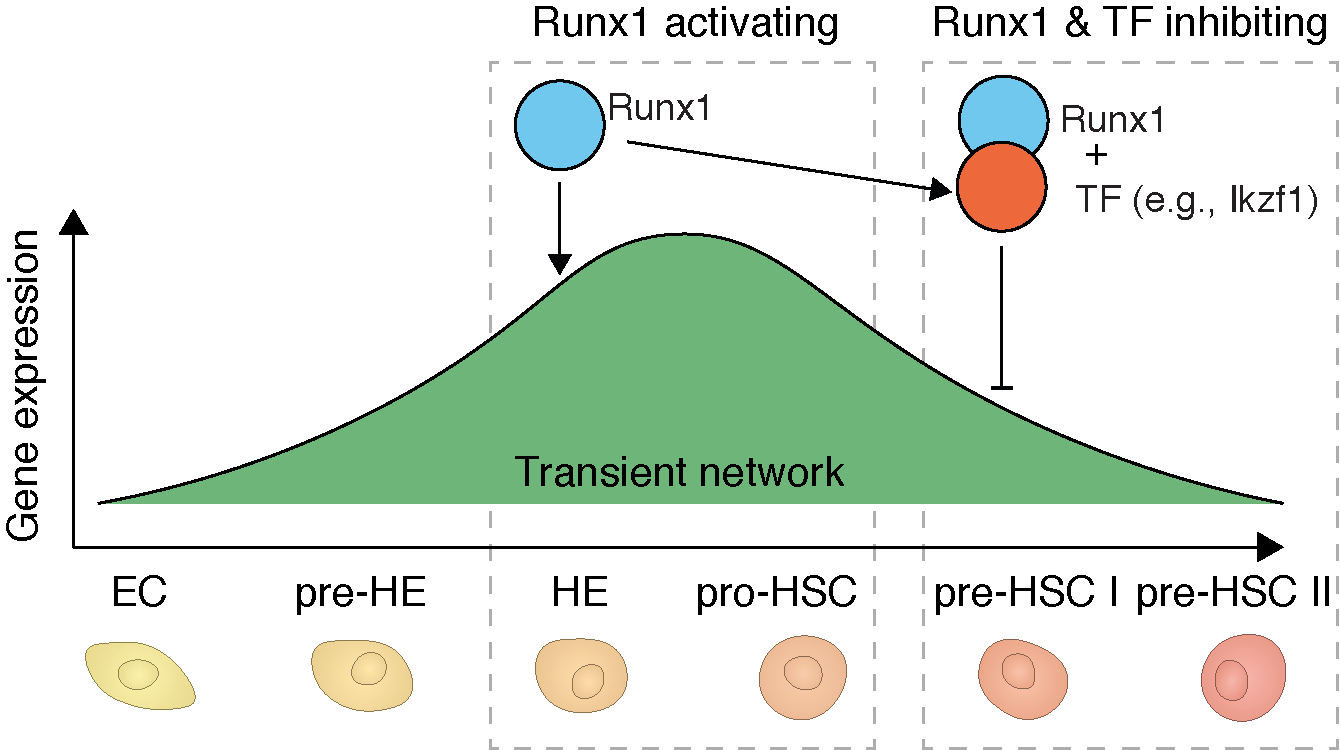
\includegraphics[width=\textwidth,height=\textheight,keepaspectratio]{figures/models/ch6_model-runx1-transient.png}
    \caption[{Hypothetical model describing Runx1 regulation of the transient EHT network.}]
    {\textbf{Hypothetical model describing Runx1 regulation of the transient EHT network.}
    A model describing the hypothesis of Runx1 regulation of the transient EHT network. \textit{Runx1} initially correlates with the expression of transiently expressed genes, and Runx1 may activate the transient network. The transient genes are downregulated with the onset of late-EHT genes, such as \textit{Ikzf1}. As preliminary evidence suggests Runx1 activity swaps to repression when \textit{Ikzf1} is expressed (Appendix \ref{fig:app_notch-ffl-validation}), this could indicate a mechanism by which late-EHT TFs alter Runx1 activity to then deactivate the transient network.
    }
    \label{fig:ch6_model-runx1-transient}
\end{figure}

This strategy identified multiple TFs predicted to co-interact with Runx1, with the potential to set up FFLs. These included Ikzf1, Ets1, Meis1, Nfe2, PU.1, Mef2c, Gfi1, Pbx1, and Cebpb. These TFs were associated with motifs enriched for different modules of the GRN, such as a Meis1 and Nfe2 motif bias for endothelial enhancers (ATAC2), which might suggest that Runx1:Meis1 and Runx1:Nfe2 FFLs regulate an endothelial program. A number of these co-interacting factors were associated with motifs enriched in transiently accessible enhancers, such as Mef2c, Gfi1, and Ikzf1, suggesting these factors regulate the transient network. Taking the Notch pathway as a key transient process, I identified a Runx1:Ikzf1:\textit{Hes1} repressive FFL, where Runx1 and Ikzf1 are predicted to act cooperatively (section \ref{ch3:notch}, p.\pageref{ch3:notch}). Existing literature suggests a physical interaction between Runx1 and Ikzf1 \citep{zhou_runx_2019}, and data from L. Greder (de Bruijn lab, unpublished) indicate that Runx1 swaps from an activating TF, to repressive when \textit{Ikzf1} is expressed (Appendix \ref{fig:app_notch-ffl-validation}). This could be extrapolated as a general mechanism in which Runx1 behaviour is altered. It is possible that in early-EHT Runx1 is an activator, correlating with the onset of the transient EHT network (section \ref{ch3:profiling}, p.\pageref{ch3:profiling}). Runx1 could promote the transient expression of genes, such as \textit{Hes1}, and as Runx1 drives the expression of late-EHT genes (i.e., \textit{Ikzf1}), Runx1 activity may switch to repressive, subsequently inhibiting the transient network (Fig. \ref{fig:ch6_model-runx1-transient}). This cooperative behaviour may also exist for other Runx1 co-interacting TFs, such as Mef2c, which is also associated with a motif highly enriched in transiently accessible enhancers. While this is based on observational data and has not been extensively tested, it is an interesting hypothesis that could suggest a previously unappreciated role in Runx1 control of EHT.

In \textit{MLL}r leukaemia, TF cooperation was investigated by exploring how RUNX1 and MYB co-regulate targets in the context of MLL-AF4 binding. RUNX1 and MYB were found to function together to increase expression of \textit{BCL2} and \textit{MYC} (section \ref{ch4:tf-cointeraction}, p.\pageref{ch4:tf-cointeraction}). MLL-AF4 is the primary driver of \textit{MYC} and \textit{BCL2} expression, but the cooperative action of RUNX1 and MYB incrementally increased expression of these loci. As it also appears that MLL-AF4 encourages the binding of TFs (section \ref{ch4:ma4-runx1-cor}, p.\pageref{ch4:ma4-runx1-cor}), it indicates that MLL-AF4 functions cooperatively with multiple TFs, and highlights the importance of incremental TF activity underpinning MLL-AF4 target genes.

%\section{Regulation of Runx1 in a pre-HE state}
%An additional interesting observation in EHT was the investigation of the pre-HE cell type. 
%<Brief CD109>
%<Runx1 + 23 regulators>

\section{The deregulation of normal GRNs in \textit{MLL}r leukaemia.}

One of the main questions asked in this thesis is "how are normal circuits altered in disease?" This was largely addressed through analysis of MLL-AF4 ALL and MLL-AF9 AML GRN models in chapters \ref{chapter4_MA4} and \ref{chapter5_normToLeuk}. The analysis in these chapters hint towards several possible mechanisms by which MLL-FPs could transform a normal function network. For instance, MLL-AF4 binding and spreading increases the frequency of RUNX1 and MAZ binding (section \ref{ch4:ma4-runx1-cor}, p.\pageref{ch4:ma4-runx1-cor}). This appears to be mediated through increased affinity for existing TF DNA binding, which may be driven through MLL-AF4 altering the chromatin environment. This could be a general principal for all TFs, whereby MLL-AF4 co-opts the activity of existing TFs and directs their activity to MLL-AF4 targets. As such, this provides a novel model for how MLL-AF4 sets up novel disease-specific interactions by altering the chromatin environment (Fig. \ref{fig:ch6_model2}).

\begin{figure}[!t]
    \centering
    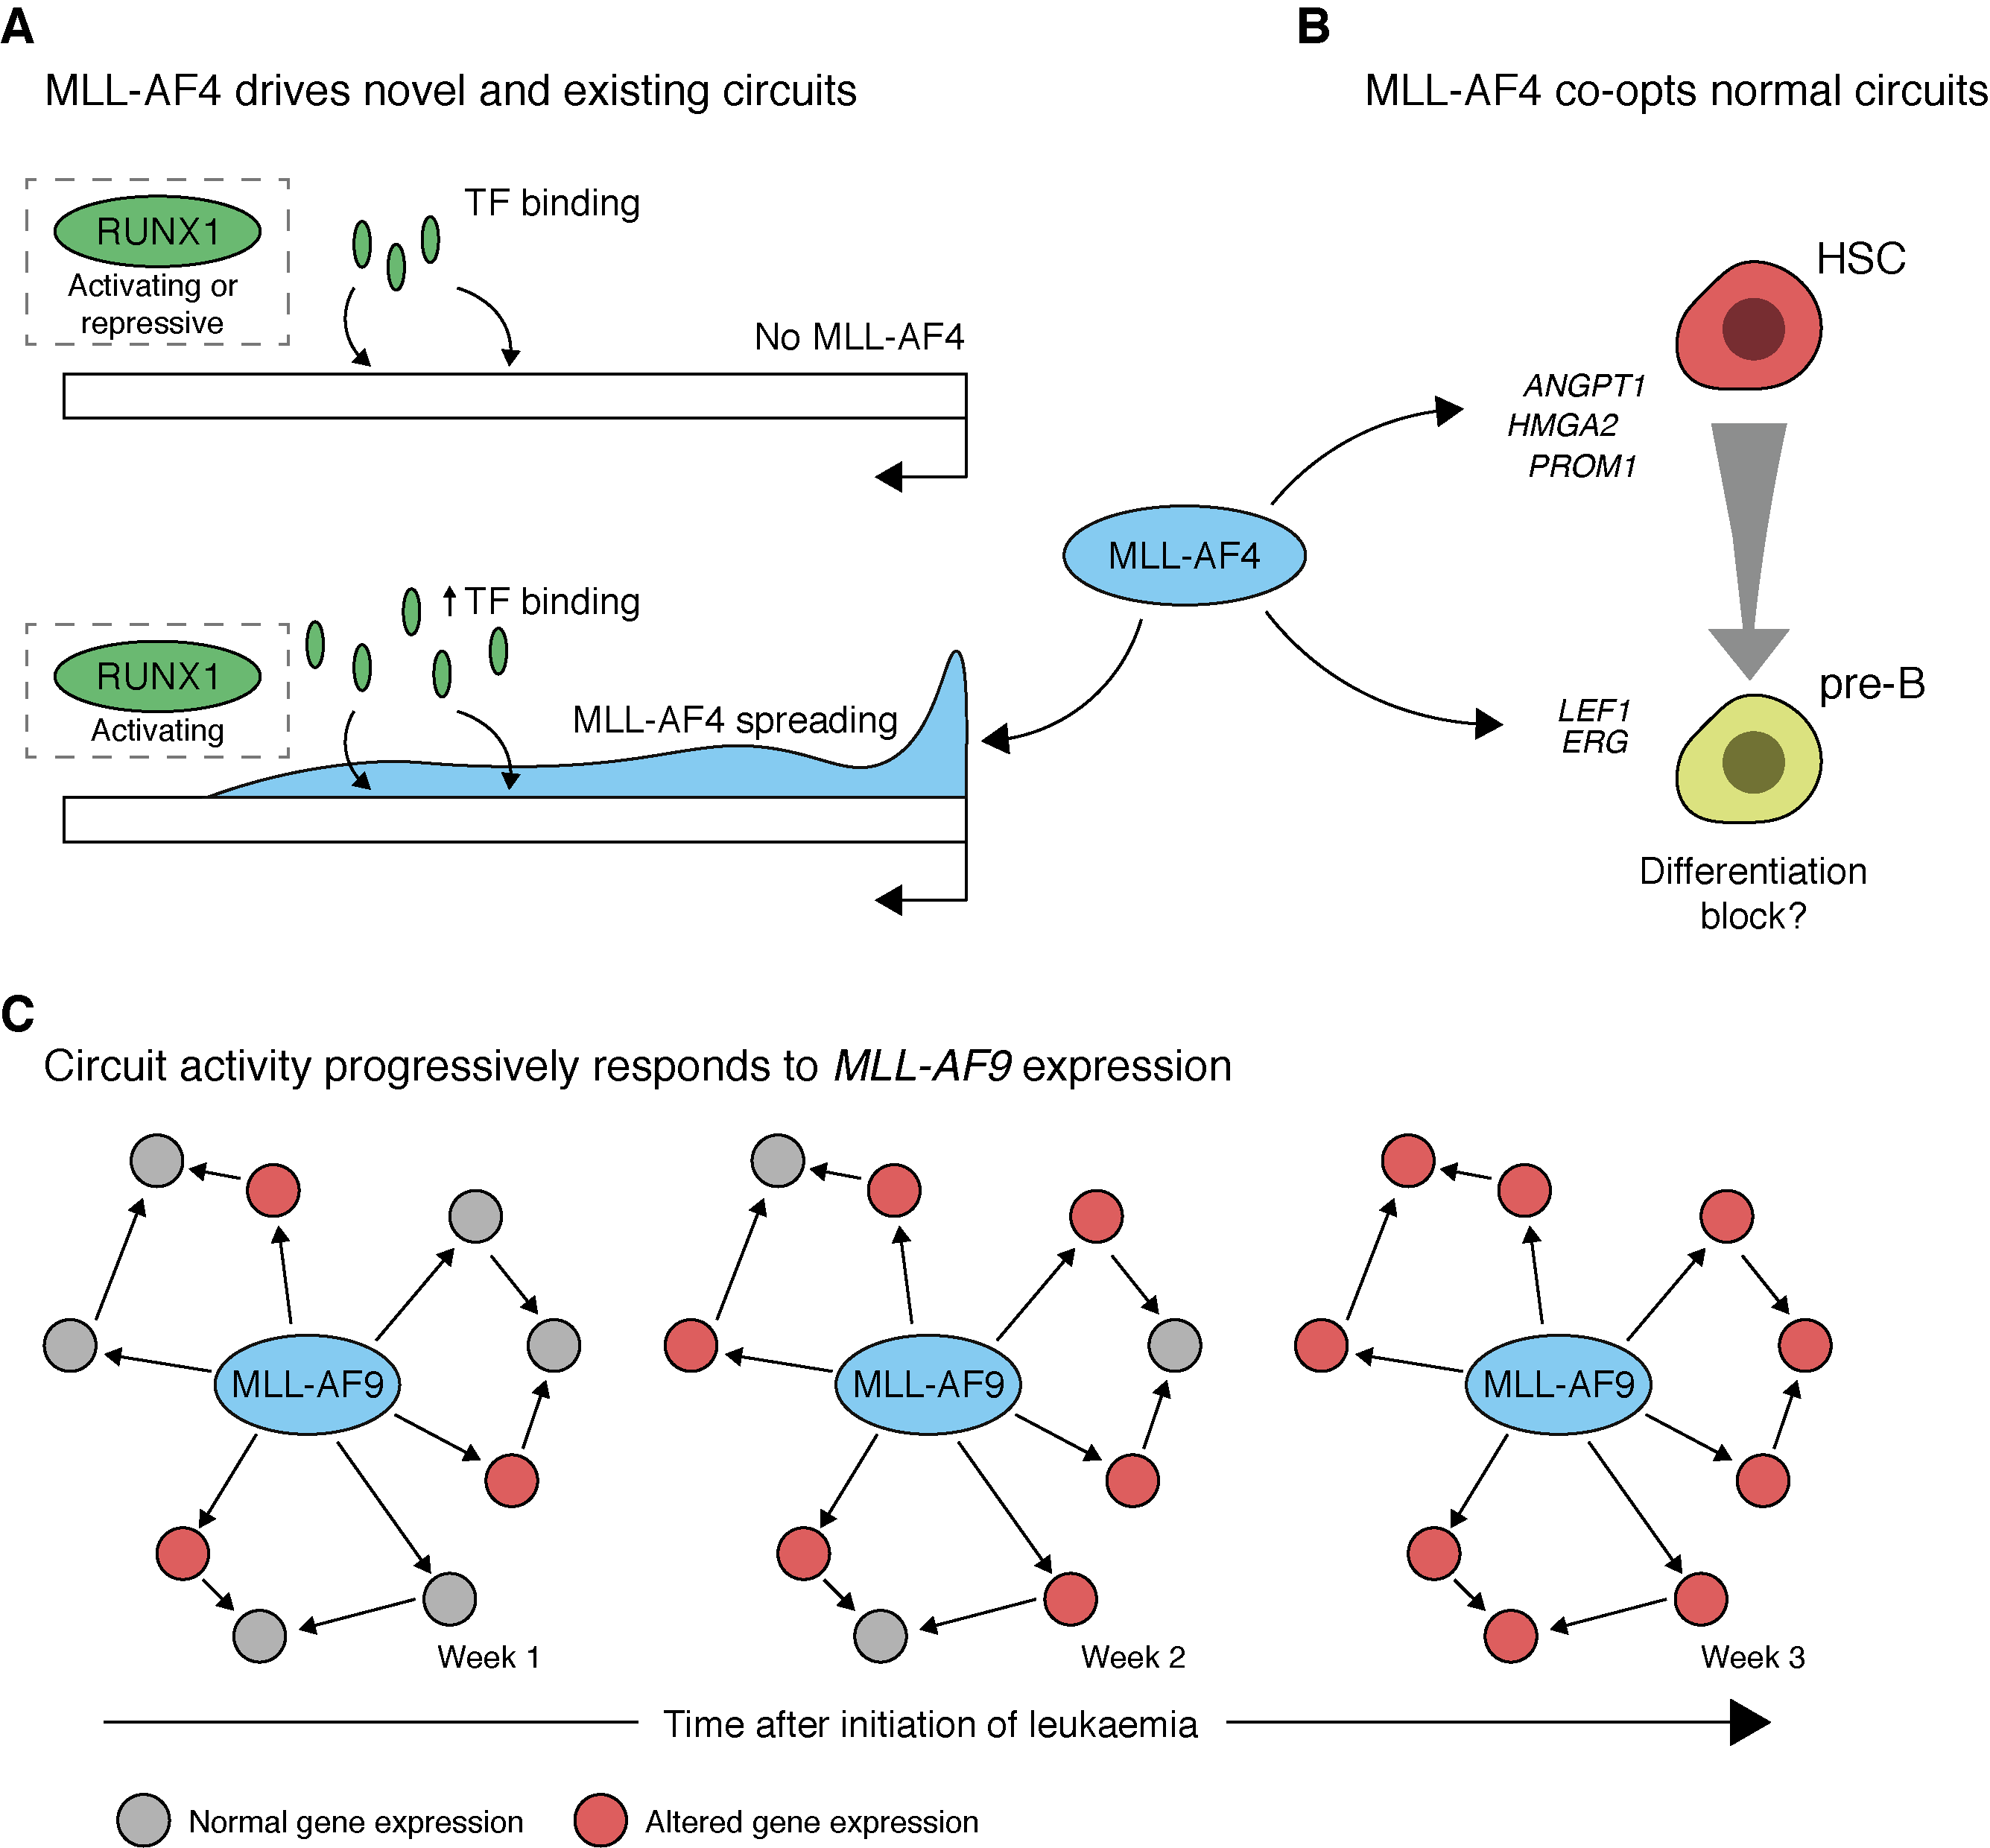
\includegraphics[width=\textwidth,height=\textheight,keepaspectratio]{figures/models/ch6_model2.png}
    \caption[{Summary model describing possible mechanisms by which the normal GRN is affected in \textit{MLL}r leukaemia.}]
    {\textbf{Summary model describing possible mechanisms by which the normal GRN is affected in \textit{MLL}r leukaemia.}
    The impact of MLL-AF4 or MLL-AF9 on a normal transcriptional network can be described as three general concepts. 
    \textbf{(A)} First, MLL-AF4 has the potential to establish novel TF interactions and alter the activity of RUNX1. 
    \textbf{(B)} Secondly, MLL-AF4 can co-opt pre-existing normal circuits, either to reactivate early HSC expressing genes, or to forcibly maintain expression of pro-B or pre-B genes. This co-opting of circuits could be underlie the differentiation block of \textit{MLL}r ALLs. 
    \textbf{(C)} Additionally, it appears that the activity of circuits do not immediately change upon expression of \textit{MLL-AF9}, and that instead gene expression is altered over time.
    }
    \label{fig:ch6_model2}
\end{figure}

One interesting observation is that RUNX1 activity appears to change depending on the presence of MLL-AF4 (section \ref{ch4:ma4-runx1}, p.\pageref{ch4:ma4-runx1}). It was observed that at gene targets with RUNX1 but no MLL-AF4, RUNX1 both upregulated and downregulated expression. This is congruent with the known behaviour of RUNX1, which can recruit both activating and repressing cofactors \citep{yamagata_runx1aml1_2005, kitabayashi_interaction_1998, perry_runx1aml1_2002, canon_vivo_2003}. However, where MLL-AF4 is bound, RUNX1 activity is biased towards activation. This suggests that MLL-AF4 alters the activity of RUNX1, potentially in a similar fashion to the Runx1 and Ikzf1 cooperation as discussed in section \ref{ch6:coop}. This highlights the potential for MLL-AF4 to not only promote novel GRN interactions, but to alter the behaviour of TFs to further activate genes (Fig. \ref{fig:ch6_model2}).

While MLL-AF4 appears to alter the normal GRN through novel interactions and biasing TF regulatory logic, it is clear that it also co-opts and activates existing circuits. This was investigated by comparing the MLL-AF4 GRN model with fetal B lymphopoiesis signatures (section \ref{ch4:multiome}, p.\pageref{ch4:multiome}), where MLL-AF4 was predicted to interact and drive several B lymphopoiesis associated genes. \textit{ERG} is normally expressed from HSCs through to pro-B cells, and is strongly upregulated by MLL-AF4. I speculated that MLL-AF4 overexpression of \textit{ERG} expression could explain the block in differentiation seen in \textit{MLL}r ALL \citep{lin_instructive_2016}, as \textit{ERG} overexpression causes a partial pro-B to pre-B block in mice \citep{tsuzuki_promotion_2011} (Fig. \ref{fig:ch6_model2}). Additionally, this analysis noted activation of stem cell genes, such as \textit{HMGA2} and \textit{ANGPT1}, both of which have significant regulatory roles and contribute to leukaemogenesis \citep{eguchi-ishimae_hmga2_2014, guenther_aberrant_2008, zhou_hematopoietic_2015}. This highlights the capacity for MLL-AF4 to reactivate stem cell regulatory factors not normally present in pro-B cells (Fig. \ref{fig:ch6_model2}). It is interesting that in this analysis only a few stem cell genes are predicted targets of MLL-AF4, suggesting the fusion protein can only reactivate (or maintain expression, depending on the cell type the translocation event occurs) a specific subset of genes. What discriminates the targeting of these genes from others is not yet clear.

A final observation was made using the MLL-AF9 GRN, which incorporated a time course experiment following leukaemic transformation. It was noted that despite a lack of change in MLL-AF9 binding over the time course, there were significant gene expression and chromatin accessibility changes (section \ref{ch5:profiles}, p.\pageref{ch5:profiles}). This suggested that while MLL-AF9 likely binds to gene targets rapidly, the impact on gene expression is progressive. This was most striking with the observation that the transcriptome of \mybmre{} mice did not diverge from \mybwt{} mice until two weeks after leukaemia initiation. This experiment does not contain baseline levels of expression in untransformed GMPs, so the most immediate transcriptional effects are lost, however it is clear that these GRNs adapt in complex ways over time, likely due to secondary effects resulting from initial \textit{MLL-AF9} expression. 

%\subsection{MLL fusion proteins target a core set of TFs, but downstream regulation is context dependent}
%<MLL-AF4 -> RUNX1 -> context dependencies>
%<MYB system - RUNX1 appears to be repressive? MYC paper too...>

\section{Future work}

%The analyses in this thesis have suggested several mechanisms of gene regulation underlying EHT and the transformation of normal networks in disease. However, several smaller observations warrant further investigation in future studies. 

\subsection{Validating predicted interactions}

In chapter \ref{chapter3_EHT} a number of candidate drivers of EHT were predicted, including Ikzf1, Cd109, Maf and Lef1, among others. As these are predictions based on the GRN model, functional validation is necessary to draw conclusions on EHT progression. A straightforward approach to do so is to knockout these factors in mESCs, followed by haematopoietic differentiation to assay the impact on EHT. However, mESC differentiation is not a perfect model of in vivo EHT, and therefore to truly validate these drivers mouse knockout models are required. For predicted regulators of the EHT budding process, such as Maf and Lef1, it would be interesting to observe the effect of their perturbation on cytoskeletal structures. 

%The GRN model also allowed for the prediction of specific circuits, such as the Runx1:Ikzf1:\textit{Hes1} FFL. This FFL was prelimarily validated by L. Greder (Appendix \ref{fig:app_notch-ffl-validation}), though additional replicates are needed to improve confidence. 

For chapters 4 and 5 the GRN models predicted several direct and indirect targets of MLL-AF4 and MLL-AF9, that are proposed to be important for leukaemia function. These factors could simply drive survival and proliferation, but could also contribute to several additional aspects of cancer biology. For instance, while a knockout of a key TF may not impact cell growth in culture, it may affect bone marrow engraftment in transplant experiments, or alter the bone marrow niche environment as seen with \textit{ANGPT1} \citep{zhou_hematopoietic_2015}. Therefore, to truly validate the importance of key nodes in the \textit{MLL}r GRNs mouse transplants would be ideal. An interesting model of infant MLL-AF4 leukaemia has been established in \cite{rice_human_2021}, where an \textit{MLL-AF4} translocation can be induced CD34+ FL cells via CRISPR Cas-9, then transplanted into mice. Using this model to assay specific TF perturbations would be a convincing validation of the importance of these key nodes. 

\subsection{Investigating TF cooperativity}

Several cases of TF cooperativity have been proposed, such as where Runx1 cooperation with Ikzf1 and MLL-AF4 is implied to change Runx1 activity, and warrants further investigation. A system developed by \cite{blackledge_variant_2014} can be used to study protein interactions in mESCs, referred to as the Tet repressor (TetR) system. TetR mESCs have an inserted Tet operator (TetO) array embedded in a 170 kb gene desert. By expressing \textit{TetR} fused to a gene of interest, the resulting TetR:protein fusion binds to the transcriptionally inactive TetO, allowing us to probe the recruitment of cofactors. By generating TetR:Runx1 fusions, alongside expression of \textit{Ikzf1}, the recruitment of cofactors can be investigating in the context of Ikzf1 activity. Alternatively, the perturbation studies can be redesigned. Knockout and siRNA knockdown experiments involve perturbation treatments lasting at least multiple days, or even incomplete removal of protein. The dTAG system involves fusing a FKBP\textsuperscript{F36V} to the N- or C-terminus of a protein of interest, then upon treatment with small molecule dTAG-13, the protein-FKBP\textsuperscript{F36V} fusion is targeted by the CRBN E3 ligase complex and rapidly degraded \citep{nabet_dtag_2018}. This can be used to rapidly degrade Runx1, Ikzf1, or MLL-AF4, and allow us to determine the impact of specific circuits on gene regulation in a much shorter time frame, thus presenting cleaner evidence of TF cooperation dynamics in FFLs with fewer secondary effects following perturbation.

\subsection{Improving GRN analyses}

The analysis in chapter \ref{chapter5_normToLeuk} is largely preliminary, and additional work is required to fully investigate this system. For instance, an important caveat for this chapter is that the Myb TF has a short core motif (5'-AACNG-3', \cite{ogata_solution_1994}), which results in an abundance of matching DNA sequences across the genome. The data could therefore benefit from Myb ChIPmentation for stronger evidence of Myb binding. Additionally, the analysis has strongly focused on just a few gene expression modules that highlight overexpression in \mybwt{} over \mybmre{} genotypes, and an exploration of the wider GRN could reveal interesting mechanisms of GRN evolution over time.

In general, there are a number of additional GRN methodologies that could be applied to the systems studied in this thesis. More advanced alternatives to measures of centrality have been developed that attempt to measure the influence of a node (node influence metric). One example is the measure of "expected force" \citep{dunn_use_2005, girvan_community_2002}, which quantifies the information spreading potential of each GRN node. Additionally, more advanced network-based methods of identifying specific GRN modules could be applied, as opposed to clustering based on gene expression patterns. For example, the edge-betweenness approach applies the betweenness centrality calculation to edges rather than nodes, then high betweenness edges are iteratively deleted, until distinct, disconnected networks are established. This is an alternative method to identify complex structures in the GRN models, and could highlight circuits underpinning key processes that have otherwise been missed using a gene expression clustering approach.

Gene regulation studies have increasingly moved towards single-cell based approaches, with recent technological advancements allowing both RNA and ATAC-seq simultaneous profiling. The use of single cell approaches for development of networks is an exciting prospect, as specific circuits may exist in particular cell types, or expression of TFs may be stochastic or oscillate, which single cell resolution assays may offer insight into. The RNA+ATAC multiome data used in section \ref{ch4:multiome} p.\pageref{ch4:multiome} could be used to establish both ALL and normal B-lymphopoiesis GRN models. Tools have been developed to create GRN models from these data, such as the recently updated SCENIC+ package \citep{gonzalez-blas_scenic_2022}. Additionally, Perturb-seq is a single cell approach that has been developed to integrate a genome wide CRISPR screen paired with gene expression profiling \citep{dixit_perturb-seq_2016, }, thus allowing the impact of many gene perturbations on the surrounding network. This has been applied recently to the K562 cell line (chronic myeloid leukaemia) \citep{replogle_mapping_2022}, establishing a genome wide genotype-phenotype map, that could be a strong resource for establishing GRN models. The use of these single cell methods is an exciting prospect, and could offer insights into the dynamics of GRN circuits at a single cell resolution.


%\subsection{Improving GRN analyses}


% https://www.ncbi.nlm.nih.gov/pmc/articles/PMC6776849/ FIMO Good, ensemble better...


%\subsection{Modelling small-scale circuits}
%<Integrate biochemical assays for small, key circuits>


